\section{Two body problem con l'atomo d'idrogeno}
Si parte da un sistema con due particelle inizialmente indipendenti, provviste di massa, posizione e carica. Si ha anche un potenziale che dipende solo dalla distanza tra le due particelle: $\hat V(|r_1 - r_2|)$. \\
L'Hamiltoniana del sistema è $\H = \frac{\vhat P_1^2}{2m_1} + \frac{\vhat P_2^2}{2m_2} + \hat V(|r_1 - r_2|)$. Abbiamo gli operatori momento $\hat p_i$ lungo gli assi e gli operatori posizione $\hat x, hat y, hat z$, per ogni particella. Si hanno le usuali proprietà di commutazione, più il fatto che gli operatori della prima particella commutano sempre com quelli della seconda.

Ora è possibile effettuare il seguente cambio di parametri:
\[
\begin{cases}
    \vhat R = \frac{m_1\vhat r_1 + m_2\vhat r_2 }{M} \\
    \vhat r = \vhat r_1 - \vhat r_2
\end{cases}\ ,\ \ 
\begin{cases}
    \vhat P = \vhat p_1 - \vhat p_2
    \vhat p = \frac{m_2\vhat p_1 - m_1\vhat p_2}{M} \\
\end{cases}
\]
Dove $M$ è la somma delle masse. Si chiama $\mu$ la massa ridotta.
Si hanno regole di commutazione solite anche per queste nuove coppie. La nuova Hamiltoniana è:
\[
    \H = \frac{\vhat P^2}{2M} + \frac{\vhat p^2}{2\mu} + V(|\vhat r|)
\]
A questo punto si ha che l'Hamiltoniana è separabile in due Hamiltoniane come segue:
\[
    \H_{cm} = -\frac{\hslash}{2M} \Lap_{\vec R} \ , \ \ \ \H_{rel} = -\frac{\hslash}{2\mu} \Lap_{\vec r} + V(|\vec r|)
\]
% Grazie alle nozioni introdotte nei capitoli precedenti per quanto riguarda il prodotto di spazi di Hilbert possiamo dire 

Nella base delle energie l'equazione di Schrödinger diventa:
\[
    \H = \psi(\vec R, \vec r) = E \psi(\vec R, \vec r)
\]
al ché
\[
    \psi(\vec R, \vec r) = \CHI(\vec R) \vphi(\vec r)
\]
ed $E = E_{cm} + E_{rel}$. Siccome entrambe queste funzioni rispettano l'equazione di Schrödinger:
\[
    -\frac{\hslash^2}{2M} \Lap_{\vec R} \CHI(\vec R) = E_{cm} \CHI(\vec R) \]\[
    \CHI(\vec R) = \fourierconst[3] e^{\frac{i}{\hslash}(\vec P \cdot \vec R)}
\]
Invece per $\vphi$:
\[
    -\frac{\hslash^2}{2M} \Lap_{\vec r} \vphi(\vec r) + V(|vec r|) = E_{r} \vphi(\vec r)
\]
Questo problema è risolvibile tramite passaggio alle coordinate polari:
\[
    \begin{cases}
        r = \sqrt{x^2 + y^2 + x^2} \\
        \theta = \arccos (\frac{z}{r}) \\
        \phi = \arctan (\frac{y}{x})
    \end{cases}
\]
L'equazione di Schrödinger diventa:
\[
    \frac{1}{r^2} \deriv[r]{} \l r^2 \deriv[r]{\vphi} \r + \frac{1}{r^2 \sin(\theta)}\left[ \sin (\theta) \sderiv[\theta]{\vphi} + \cos (\theta) \deriv[\theta] {\vphi} \right] + \frac{1}{r^2 \sin^2(\theta)} \sderiv[\phi]{\vphi} + \frac{2 \mu}{\hslash^2}(\varepsilon - V(r))\vphi(r,\theta,\phi) = 0
\]
che qeuivale a :
\[
    \frac{1}{R}\deriv[r]{}r^2 \deriv[r]{R} + \frac{2\mu r^2}{\hslash^2}(\varepsilon - V(|r|)) + \frac{1}{y \sin (\theta) \deriv[\theta]{} \sin\theta \deriv[\theta]{y}} + \frac{1}{\sin^2 \theta} \sderiv[\phi]{y} + \lambda = 0
\]
Dove la $y$ è scrivibile come $A(\theta) B(\phi)$, chiamate componente radiale e componente azimutale. Al ché:
\[
\frac{\sin \theta}{A}\deriv[\theta]{}(\sin\theta \deriv[\theta]{A}) = - \lambda \sin^2 \theta \frac{1}{B} \sderiv[\phi]{B} = \eta
\]
dove $\eta$ è una variabile di calcolo. Si ha chiaramente che $B$ è periodica di periodo $2\pi$, ed è della forma:
\[
B'' + \eta B = 0
\]
quindi con semplici calcoli si ottengono due casi: per $\eta = 0$ si ha $B = \fourierconst[1] \phi$. Per $\eta < 0$ non esistono soluzioni. Per $\eta > 0$ si può derivare che $B_\eta = \fourierconst[1] e^{1\sqrt \eta \phi}$, valida solo quando $\sqrt \eta$ è intero (calcoli per esercizio). Si può quindi generare una base $B_n = \frac{e^{im\phi}}{\fourierconstinv[1]}$.

Per quanto riguara la componente radiale $A$ si ha, chiamando $\xi = \cos\theta$:
\[
\deriv[\xi]{} \l (1-\xi^2)\deriv[\xi]{A} \r + (\lambda - \frac{m^2}{1-xi^2})A=0
\]
A seguito di un ulteriore cambio $A(\xi) = (1-\xi^2)^{|m|/2}f(\xi)$:
\[
\l 1-\xi^2 \r f'' - 2 \l |m| + 1 \r \xi f' + \left[ \lambda - |m|(|m| + 1) \right] f = 0
\]
che è un'equazione differenziale fuxiana. Al ché si pone quindi $f(\xi) = \sum_{s = 0}^{\infty} c_s\xi^s$ e si ottiene:
\[
    f'(\xi) = \sum_{s = 0}^{\infty} sc_s\xi^{s-1}\ ,\ \ \ f''(\xi) = \sum_{s = 0}^{\infty} s(s-1)c_s\xi^{s-2}
\]
e risulta:
\[
    \sum_{s = 0}^{\infty} (s+1)(s+2)c_s\xi^{s} - \sum_{s = 0}^{\infty} s(s+1)c_s\xi^s-2(|m| + 1) \sum_{s = 0}^{\infty} sc_s\xi^s + \left[ \lambda - |m| (|m| + 1) \right] \sum_{s = 0}^{\infty} c_s\xi^s = 0
\]
al ché si possono porre uguali a zero tutte le somme dei coefficienti, grado per grado:
\[
    c_2 = \frac{c_0}{2} \left[ \lambda - |m|(|m| + 1) \right]c_0 = 0 \] \[
    c_3 = \frac{c_1}{6}\left[ 2(\abs m + 1) - \lambda + \abs m (\abs m + 1) \right] \]\[
    c_{s+2} = c_s \frac{1}{(s+1)(s+2)} \left[ (s+\abs m) (s + \abs m + 1) - \lambda \right]
\]
Si può notare anche un fatto importante: coefficienti di indice dispari generano funzioni dispari, e coefficienti pari generano funzioni pari. Al ché si può ulteriormente suddividere $f(\xi) = c_0 F(\xi^2) + c_1 \xi G(\xi^2)$. Tuttavia è necessario ricordare del polo in $\xi = 0$ che si aveva nell'espressione di prima. Bisogna quindi imporre che $f$ sia regolare per $\xi = \pm 1$, che è vero se e solo se il raggio di convergenza della serie è $\geq 1$:
\[
    r_c = \lim_s \frac{\abs{c_s}}{\abs{c_{s+2}}} = \lim_s \frac{(s+1)(s+2)}{(s+\abs m)(s + \abs m + 1) - \lambda} = 1
\]
A questo punto possiamo porre $\lambda$ in modo che esista un $\nu$ intero tale che $\lambda = (\nu + \abs m)(\nu + \abs m + 1)$. Questo fa sì che la successione
\[
c_{s+2} = c_s \frac{1}{(s+1)(s+2)} \left[ (s+\abs m) (s + \abs m + 1) - \lambda \right]
\]
è definitivamente nulla, quindi la $f$ diventa un polinomio di grado $\nu$! Chiamiamo ora $l = \nu - \abs m$:
\[
    A_l^{|m|} (\theta) = (1 - \xi^2)^{|m|/2}f_{l-\abs m}(\xi)\ ,\ \ \ \xi = \cos(\theta)
\]

% e imponendo la normalizzazione di $\vphi$:
% \[
%     \sfabs{\vphi} = 1 = \rint \abs{\vphi(\vec r)} d\vec r
% \]


% --------------------------- 5 Dicembre --------------------------------

Ora, dal nulla è comparsa l'equazione seguente:
\[
    (1-\xi)^2f'' - 2 \xi f' + l(l+1)f = 0
\]
che è un'equazione di Legendre, le cui soluzioni sono composizioni dei polinomi di Legendre definiti come:
\[
    P_l(\xi) = (-1)^l\frac{1}{2^l l!} \frac{\partial^l}{\partial \xi^l}(1-\xi^2)^l
\]
Brutto forte neh?

Vabè ora abbiamo le armoniche sferiche $Y_l^m(\theta, \phi) = C_{lm}e^{im\phi}P_l^m(\cos \theta)$ con:
\[
    P_l^m(cos \theta) = C_l^{\abs m}(-1)^m(\sin \theta)^{\abs m} \frac{\partial^{\abs m}}{\partial \xi^{\abs m}}P_l(\cos \theta)
\]

Ora che sappiamo la componente angolare per \textbf{ogni} problema a potenziale radiale, possiamo tornare alla componente radiale dello stato:
\[
    \frac{1}{r}\sderiv[r]{}(rR)+\frac{2\mu}{\hslash^2}\left[ \varepsilon - V(r) - \frac{\hslash^2 l (l+1)}{2\mu r^2} \right] R = 0
\]
dove la terza componente $\frac{\hslash^2 l (l+1)}{2\mu r^2}$ è il potenziale centrifugo. Bisogna notare che da quest'ultima equazione si deriva che $R$ è della forma $R_l^n$, dove $l$ è il numero quantico orbitale e $n$ il livello energetico.

Mettendo assieme quanto trovato risulta che $\phi$ è della forma:
\[
    \vphi_{nlm}(r, \theta,\phi ) = R_{nl}(r)Y_l^m(\theta, \phi)
\]

\subsubsection*{Applicazione sull'atomo d'idrogeno}
I dati sono:
\[
    \begin{cases}
        m_p = 1.7\ 10^{-30}kg\\
        m_e = 0.56\ 10^{-27}kg\\
        e^- = 1.6\ 10^{-19}C\\
    \end{cases}
\]
Si inizia definendo alcuni parametri comodi:
\[
    \begin{cases}
        E_0 = \frac{\mu e^4}{2\hslash^2}\\
        a_0 = \frac{\hslash}{\mu e^2}
        \rho = \frac{r}{a_0} \\
        \lambda = \sqrt{\frac{-\varepsilon}{E_0}}\\
        y = rR
    \end{cases}
\]
Il potenziale utilizzato è $V(r) = \frac{e^2}{r}$, e dai ragionamenti di prima si trova l'equazione differenziale per la componente radiale:
\[
    \sderiv[\rho]{y} - \frac{l(l+1)}{\rho^2}y + \frac{2}{\rho}y - \lambda^2\mu = 0
\]
Introduciamo $u = e^{\lambda \rho}y$, al ché:
\[
    u'' - 2\lambda u'+ \l \frac{2}{\rho} - \frac{l(l+1)}{\rho^2} \r u = 0
\]
Supponiamo $u$ della forma $u = \rho^2 \sum_i c_i\rho^i$, dove $s$ è un coefficiente intero positivo tale che $u$ va a 0 più velocemente di BOH. \\
Procediamo come con l'equazione fuxiana di prima:
\[
    \sum_i c_i (i+q)(i+s-1)\rho^{i+s-2} - 2\lambda \sum_i c_i (i+q)\rho^{i+s-1} + 2  \sum_i \l c_i \rho^{i+s-1} - l(l-+1)\rho^{i+s-2} \r = 0
\]
Risulta, per i primi gradi:
\[
    \begin{cases}
        c_0 \l s(s-1) - l(l+1) \r = 0\ \ \implies\ \ s = l + 1  \\
        c_i = 2c_{i-1}\frac{\lambda (i+l) - 1}{i(i+2l+1)}
    \end{cases}
\]
con $c_0$ libero. Affinché la $u$ sia $\L^p$ deve essere convergente ovunque, quindi serve che:
\[
    \lim_i \frac{c_i}{c_{i-1}} \sim \frac{2\lambda i}{i^2} = 0 \ \ \implies \ \ R_{conv} = \infty
\]
Tuttavia questo farebbe sì che la $y$ originale sarebbe sempre divergente, in quanto si può dimostrare che questa $u$ in maniera esponenziale su $\rho$; quindi è necessario che la successione $(c_i)$ sia definitivamente zero, ovvero un polinomio finito! Se l'ultimo valore non nullo della successione è $c_p$, risulta che $\lambda = \frac{1}{\bar p -+ l} = \sqrt{\frac{-E}{E_0}} = \frac{1}{n}$. Al ché $n = \bar p + l$.

Risulta infine $E_n = \frac{1-\mu e^4}{2\hslash n^2}$ dipende da solo $n$ e non da $l$: questo fenomeno è chiamato \textbf{degenerazione accidentale}\index{Degenerazione accidentale}.\\
Componendo il tutto risulta quindi: 
\[
    y_{nl} = e^{-\lambda_n \rho} u_{nl}(\rho) = e^{-\frac{\rho}{\bar p+l}} \rho^{l+1} \sum_{i=0}^{\bar p} c_i \rho^i \]\[
    R_{nl}(\rho) = \frac{y_{nl}}{\rho}
\]
Ora vediamo cosa accade per $l = 0$ e $n$ piccoli:
\[
    \begin{cases}
        R_{10} = 2(a_0)^{-3/2}e^{-r/a_0} \\
        R_{20} = 2(2a_0)^{-3/2} \l 1 - \frac{r}{2a_0} \r e^{-r/2a_0} \\
        R_{21} = \frac{(2a_0)^{-3/2}}{\sqrt 3} \frac{r}{a_0} e^{-r/2a_0}
    \end{cases}
\]
Al ché, componendo tutto:
\[
    \vphi(\theta, \phi) = \frac{2}{na_0} \frac{(n-l-1)!}{2n\l (n+l)! \r^3}e^{-r/na_0} \l \frac{2e}{na_0} \r L_{n+l}^{2l+1}(\frac{2r}{na_0}) Y_l^m(\theta, \phi)
\]
dove i $L_{n+l}^{2l+10}$ sono le funzioni associate di Laguerre. Si ricorda che le restrizioni sui pedici sono:
\[
\begin{cases}e^{-r/a_0}
    n\ \rightarrow l = 0, \cdots, n-1 \\
    l\ \rightarrow m = -l, \cdots, l \\
\end{cases}
\]
Si definisce la \textbf{degenerazione}\index{degenerazione} degli stati, ovvero quanto aumentano di numero le autofunzioni allo stato eccitato $n$. Risulta che la degenerazione è $n^2$, infatti:
\[
   n = 1\  \rightarrow \ \begin{cases}
        \vphi_{100}
    \end{cases}, \ \ 
   n = 2\  \rightarrow \ \begin{cases}
        \vphi_{200} \\
        \vphi_{21-1} \\
        \vphi_{210} \\
        \vphi_{211}
    \end{cases}, \ \ \cdots
\]
I polinomi di Laguerre sono definiti come segue:
\[
    L_i (\rho) = e^{\rho} \nderiv[\rho]{}{i}(\rho^i e^{-\rho})
\]
e le funzioni associate sono:
\[
    \L_i^s(\rho) = \nderiv[\rho]{}{s}L_i
\]

Risultano comodi i diagrammi polari, in cui si trascura la componente data dalle funzioni associate.
\begin{center}
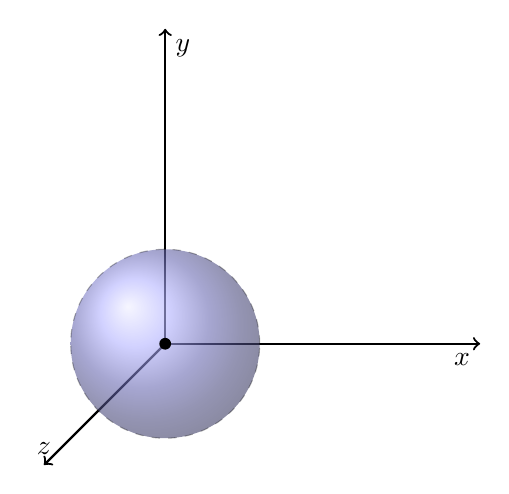
\begin{tikzpicture}[scale=2]
    % Draw axes
    \draw[thick,->] (0,0,0) -- (2,0,0) node[anchor=north east]{$x$};
    \draw[thick,->] (0,0,0) -- (0,2,0) node[anchor=north west]{$y$};
    \draw[thick,->] (0,0,0) -- (0,0,2) node[anchor=south]{$z$};
    
    % Draw spherical orbital (S orbital - spherically symmetric)
    \shade[ball color=blue!40, opacity=0.6] (0,0,0) circle (0.6cm);
    
    % Optional: add contour lines for better visualization
    \draw[dashed, opacity=0.3] (0,0,0) circle (0.6cm);
    
    % Mark origin
    \node at (0,0,0) [circle, fill, inner sep=1.5pt] {};
\end{tikzpicture}
\end{center}

\begin{center}
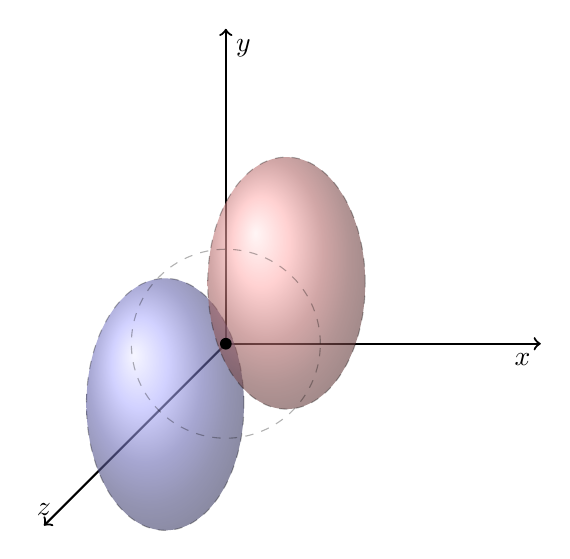
\begin{tikzpicture}[scale=2]
    % Draw axes
    \draw[thick,->] (0,0,0) -- (2,0,0) node[anchor=north east]{$x$};
    \draw[thick,->] (0,0,0) -- (0,2,0) node[anchor=north west]{$y$};
    \draw[thick,->] (0,0,0) -- (0,0,3) node[anchor=south]{$z$};
    
    % Draw P orbital lobes along z-axis
    % Upper lobe (positive z)
    \shade[ball color=blue!40, opacity=0.6] (0,0,1) ellipse (0.5cm and 0.8cm);
    \draw[dashed, opacity=0.3] (0,0,1) ellipse (0.5cm and 0.8cm);
    
    % Lower lobe (negative z)
    \shade[ball color=red!40, opacity=0.6] (0,0,-1) ellipse (0.5cm and 0.8cm);
    \draw[dashed, opacity=0.3] (0,0,-1) ellipse (0.5cm and 0.8cm);
    
    % Nodal plane at origin
    \draw[dashed, opacity=0.3] circle (0.6cm);
    
    % Mark origin
    \node at (0,0,0) [circle, fill, inner sep=1.5pt] {};
\end{tikzpicture}
\end{center}

Ora analizziamo la densità di probabilità in funzione del raggio:
\[
    \P(r, r+dr) dr = r^2 \abs {R_{10}}^2 dr = \frac{4r^2}{a_0^2} e^{-2r / a_0}
\]

Risulta che il massimo è in $r = a_0$, che è chiamato il \textbf{raggio di Bohr}\index{Raggio di Bohr}.